\documentclass[a4paper,12pt]{report}

\usepackage[a4paper]{geometry}
\usepackage{amssymb,amsmath,amsthm}
\usepackage{graphicx}
\graphicspath{ {./images} }
\usepackage{url}
\usepackage{hyperref}
\usepackage{epsfig}
\usepackage[italian]{babel}
\usepackage{setspace}
\usepackage{tesi}
\usepackage{makeidx}
\usepackage{caption, float}
\usepackage{indentfirst}

% per le accentate
\usepackage[utf8]{inputenc}
\begin{document}
\setcounter{secnumdepth}{5}
\setcounter{tocdepth}{5}

\title{Un'applicazione web per dimostrare le proprietà degli algoritmi di label propagation}
\author{Andrei Georgiani TALPALARU}
\dept{Corso di Laurea in Informatica} 
\anno{2019-2020}
\matricola{942824}
\relatore{Prof. Paolo CERAVOLO}
\correlatore{Dr. Samira MAGHOOL}

\beforepreface
\prefacesection{Ringraziamenti}
Ringrazio molto il Professore Paolo Ceravolo per avermi permesso di lavorare su questo progetto, da cui ho imparato tante nuove tecnologie su cui non ho avuto modo di mettere mano fino ad ora. 

Ringrazio anche la mia famiglia, che mi ha sostenuto per tutto questo tempo.
\afterpreface
% 
% 
%		
\chapter{Introduzione}
%/
%

\chapter{Social Network Analysis (da aggiungere piu informazioni a ogni sezione)}
	La Social Network Analysis e l'analisi delle strutture sociali attraverso le reti e la teoria dei grafi. \cite{snaintro}
	Grazie ad una rappresentazione astratta, dove le connessioni tra certi elementi di un sistema, chiamati anche nodi o agenti (quando sono capaci di fare scelte o azioni attive), la SNA puo essere applicata a una varieta di domini. Il comportamento del sistema, in termini di communicazione, propagazione ed evoluzione delle connessioni e catturato da metriche di SNA. \cite{avpra}

	\section{Reti}
	Una rete e composta da due componenti di base: i nodi e gli archi. Usando questi due componenti si possono descrivere una multidudine di strutture e relazioni (per esempio connessioni sociali, connessioni in una rete di computer, reti elettriche \dots). 

	 I nodi sono le entita presenti nella rete e che possono avere proprieta interne (per esempio un valore che rappresenta il grado del nodo, o il peso o una posizione nella rete). 

	Gli archi sono le connessioni tra i nodi che possono avere a loro volta delle proprieta (per esempio un peso o un'altro tipo di relazione tra i nodi collegati alle estremita dell'arco).	\cite{snaintro} 


	\section{Label Propagation}
	Label Propagation rappresenta una famiglia di algoritmi usati per preddire le ettichete dei nodi di una rete. 
	Differisce da altri algoritmi di Social Network Analysis siccome, invece di adottare una visione globale della rete, le decisioni prese dall'algoritmo sono fatte rispetto a proprieta locali, quindi gli algoritmi di Label Propagation adottano una visione locale della rete. \cite{raghavan} 

	L'idea generale e che le ettichete assegnate inizialmente ai nodi sono propagate attraverso la rete seguendo gli archi. La propagazione di un'etticheta a un nodo si basa sulle ettichete dei suoi vicini, tipicamente a un salto di distanza. Molteplici iterazioni permettono il raggiungimento di un'approssimazione del ottimo globale partendo da un ottimo locale. La complessita temporale varia tra tempo lineare ed esponenziale, dipendendo dalla densita della rete. L'approccio e naturalmente decentralizato, con passaggi singoli su ogni nodo ad ogni iterazione. \cite{avpra}
	
	\section{Algoritmi di Label Propagation}
	La scelta principale che differenzia i diversi algoritmi di Label Propagation e legata alla Update Rule. Alcune varianti della Update Rule che sono state usate nel tempo sono: il grado dei nodi, il coefficiente di clustering e la similarita strutturale.

	La limitazione principale degli algoritmi precedenti era l'impossibilita di scegliere piu di un'etticheta per ogni nodo. 

	Gli algoritmi sono stati generalizzati per permettere l'identificazione di communita sovrapposte. Ogni etticheta viene pesata con un belonging coefficient associato al nodo. Tutti i belonging coefficient di un nodo sommano a 1. 

	\section{Belonging Coefficient}
	Da scrivere	

	\section{AVPRA (Agent-based Vector-label PRopagation Algorithm)}
	AVPRA e un'algoritmo di Label Propagation basato su un'organizzazione ad agenti che permette di implementare la regola di update rispetto a piu fattori, come per esempio le proprieta di dominio. 

	AVPRA differisce dagli altri algoritmi tramite il fatto che l'output dell'algoritmo e un vettore compatibile col formato di input usato in maggior parte degli algoritmi di Machine Learning. Il vettore ha una lunghezza fissata per tutti gli nodi e include tutte le label della rete assieme al loro belonging coefficient basato sulle proprieta strutturali della rete. 

	Il belonging coefficient nel caso di AVPRA rappresenta una misura di diffusione/accumulo delle ettichete dei nodi, dipendente dalla distanza rispetto ad altri nodi e la loro frequenza. \cite{avpra} 

		\subsection{Propagazione basata su agenti}
		Consideriamo che le ettichete possono scorrere nella rete e gli agenti possono tenere conto della loro incidenza. Gli agenti sono semi-intelligenti e agiscono rispetto alla situazione riscontrata. Possono adottare diverse strategie nella ricezione o rifiuto di un'etticheta che scorre da un nodo vicino, in concordanza con certe condizioni. In questo modo, l'algoritmo puo controllare gli effetti globali, come per esempio la condizione di terminazione.

		\subsection{Aggiornamento sincrono}
		Per agirare i conflitti nella propagazione degli aggiornamenti, in AVPRA gli agenti sono aggiornati in modo asincrono. Il vettore delle ettichete di un certo nodo a tempo $t$ sara ottenuto dai vettori delle ettichete dei vicini a tempo $t-1$. In questo modo tutti gli agenti possono aggiornarsi simultaneamente.
	
		\subsection{Inizializzazione}
		Ogni agente viene ettichetato con un vettore di $d$ dimensioni dove $d$ e la cardinalita dell'insieme $L$, dove $L$ e l'insieme delle ettichete uniche nella rete. 

		\subsection{Funzione di aggiornamento}
		La regola di aggiornamento mostra il modo in cui i vettori di ettichete sono aggiornati ad ogni iterazione. In AVPRA, la funzione di aggiornamento e:
		\begin{equation}
		VL_i [l] (t) = w_1 VL_i [l] (t-1) + w_2 \sum_{j \in \Gamma(i)} VL_j [l](t-1)
		\end{equation}

		Dove $VL_i[l](t)$ rappresenta il valore del belonging coefficient dell'etticheta $l$ nel nodo $n_i$ al tempo $t$, $w_1$ rappresenta il peso delle ettichete correntemente assegnate al nodo $n_i$, $w_2$ rappresenta il peso delle ettichete correntemente assegnate ai nodi $\Gamma(i)$ e $\Gamma(i)$ sono i vicini del nodo $n_i$.

		\subsection{Iterazione Finale}
		L'algoritmo AVPRA finisce quando il sistema raggiunge un'iterazione s nella quale i vettori di ettichete sono stazionari. Cio implica che le variazioni dei belonging coefficient devono essere minori di un parametro p che viene chiamato negligibly threshold. 
		

\chapter[Il sviluppo dell'applicazione]{Il sviluppo di un applicazione per dimostrare le proprieta dell'algoritmo AVPRA}
\label{chapter4}

	\section{Applicazioni di visualizzazione delle reti sociali}
		
		\subsection{Visualizzatore Reti Sociali con AVPRA}
		AVPRA è un'algoritmo di Label Propagation basato su Agenti.
		Il visualizzatore delle Reti Sociali per AVPRA è un'applicazione web che permette all'utente di
		eseguire e visualizzare i risultati dell'algoritmo in un modo interattivo nel browser web. \cite{avpra}
		
			\subsubsection*{I Pro}
				\begin{itemize}
					\item Ha tanti parametri che permettono all'utente di controllare il comportamento dell'algoritmo e dell'input.
					\item Permette l'esportazione della rete e delle informazioni visibili sullo schermo in formato PNG.
					\item Permette di esportare le informazioni riguardanti il grafo e il output in formato JSON.
					\item Singoli nodi possono essere selezionati in modo da poter vedere piu dettagli e misure riguardanti quel specifico nodo.
					\item Offre la possibilita di selezionare, comparare ed esportare la comparazione tra due nodi diversi della rete.
					\item Sopporta la visualizzazione di due viste diverse: Vector Label View (mostra in modo grafico la distribuzione delle label su ogni nodo) e Community View (mostra in modo grafico la divisione della rete in communita basate sulla struttura.).
					\item Mostra graficamente la divisione in communita raggruppando i nodi della stessa communita piu vicini uno all'altro.
					\item Permette all'utente di eseguire l'algoritmo per piu iterazioni e di vedere graficamente l'evoluzioni dei Vector Label nel tempo (feature specifica di AVPRA).
					\item La paletta di colori utilizzata per i label nei Vector Label puo essere modificata usando un'ulteriore file nella fase di caricamento della propria rete.
					\item Permette all'utente di selezionare un nodo specifico tramite una barra di ricerca dove si puo inserire l'id del nodo.
				\end{itemize}
						
			\subsubsection*{I Contro}
				\begin{itemize}
					\item Sopporta un solo formato di input (tre file CSV: Lista Archi, Vector Label Iniziali, Nomi Label) e due formati di output (un file pickled contenente i risultati di tutte le iterazioni dell'algoritmo e un file JSON contenente i dati della rete o la comparazione di due nodi diversi).
					\item I dataset dell'utente e i risultati delle esecuzioni dell'algoritmo su quei dataset sono tenute sul server dell'applicazione, anche se per poco tempo.
					\item Performance piu scarse nel caso venga usato con reti molto grandi.
				\end{itemize}

		\subsection{Infomap Network Navigator}
		Infomap è un'algoritmo di clustering su reti basato su Map Equation. Infomap Online è un'applicazione web che permette agli utenti di eseguire
		l'algoritmo Infomap nel browser web. \cite{mapequationsite} 
		
		Infomap Network Navigator è un'applicazione che permette di visualizzare i risultati
		dell'algoritmo in un modo interattivo. \cite{mapequationnavigatorsite} 
		
			\subsubsection*{I Pro}
				\begin{itemize}
					\item I dataset dell'utente e i risultati dell'esecuzione dell'algoritmo su quei dataset non sono mantenute sul server di Infomap Online.
					\item Ha tanti parametri per controllare il comportamento dell'algoritmo, dell'input, del output e dell'accuratezza.
					\item Sopporta tanti formati di input (Link-List, Pajek, Bipartite, Multilayer, With inter-layer links, Without inter-layer links, States) e tanti formati di output (Phyisical, State-level output, Tree, FTree, Clu, Newick, JSON). Infomap riconosce automaticamente il formato dei file dal header del file.
					\item Permette di esportare la visualizzazione in formati SVG e PNG.
					\item Permette l'esportazione del file di output.
					\item Singoli nodi possono essere selezionati in modo da vedere piu dettagli e misure riguardati il specifico nodo.
					\item Permette all'utente di selezionare un nodo specifico tramite una barra di ricerca.
					\item Visually shows communities by grouping nodes or other sub-communities in a module (Map Equation algorithm specific visualization). Mostra graficamente il raggruppamento dei nodi in communita e sotto-communita attraverso un modulo (feature specifica Map Equation).
				\end{itemize}			

			\subsubsection*{I Contro}
				\begin{itemize}
					\item L'esportazione della visualizzazione non include nient'altro oltre la rete stessa.
					\item Non offre la possibilita di vedere il modo in cui due nodi diversi della rete siano correlati.
					\item Esiste un limite sulla dimensione dei file di input che si possono utilizzare.
					\item Non esiste un modo per personalizzare la paletta di colori che viene usata nella visualizzazione.
				\end{itemize}

	\section{Sviluppo}
		Il progetto e un'applicazione web che e divisa in 2 parti:
		\begin{itemize}
		\item Frontend - la componente dell'applicazione con cui l'utente interagisce direttamente.
		\item Backend - la componente dell'applicazione con cui interagisce il frontend e che si occupa di esporre un'API che esegue le funzionalita richieste dal frontend.
		\end{itemize}
		\subsection{Funzionalita previste}
			\subsubsection{Backend}
			\begin{itemize}
				\item Dev'essere capace di eseguire l'algoritmo AVPRA dato in Python.
				\item Deve esporre un'API che:
				\begin{itemize}
					\item permette all'utilizzatore di eseguire l'algoritmo
					\item permette all'utilizzatore di controllare i parametri dell'algoritmo come numero di iterazioni, neglibility threshold, interpretazione della rete (directed, undirected), modo di propagazione delle label (da predecessori, da successori) e formula dei pesi della regola di Update.
					\item permette di ottenere i dettagli riguardanti un solo nodo ad una certa iterazione.
					\item permette di ottenere i dettagli riguardanti la relazione tra due nodi ad una certa iterazione.
					\item permette di esportare i risultati e i dettagli dell'esecuzione in un formato definito.
					\item Deve permettere all'utente di caricare ed eseguire l'algoritmo sulla propria rete usando un formato definito.
				\end{itemize}
			\end{itemize}

			\subsubsection{Frontend}
				\begin{itemize}
					\item Deve permettere all'utente di visualizzare in modo interattivo la situazione, alla iterazione corrente, della rete e dei suoi vector label.
					\item Deve implementare un modo in cui l'utente possa caricare la sua propria rete.
					\item Deve dare la possibilita all'utente di avere piu informazioni riguardo lo stato corrente di un vector label di un nodo specifico.
					\item Deve permettere di avere informazioni riguardo l'iterazione corrente e l'iterazione finale (da definire) dell'algoritmo.
					\item Deve implementare un modo in cui si possa andare avanti e indietro tra le iterazioni in modo da vedere l'evoluzione dei vector label.
					\item Deve fare possibile la visualizzazione delle communita associate alla rete.
					\item Deve permettere di selezionare 2 nodi e di vedere la situazione corrente di entrambi.
					\item Deve implementare un modo di esportare i file che si possono esportare attraverso l'API esposta dal backend.
				\end{itemize}

		\subsection{Sviluppo dell'applicazione web}

			\subsubsection{Frontend}
			Per lo sviluppo della parte Frontend dell'applicazione, contenente l'interfaccia utente e la comunicazione col backend, sono state utilizzate diverse tecnologie e librerie. \par
			Le librerie e tecnologie che sono state utilizzate sono presentate di seguito.

			\paragraph*{React.js} \par e una libreria di JavaScript che viene usata per creare in modo facile delle interfacce utente interattive. 
				I componenti piu importanti di questa libreria che sono utilizzati all'interno dell'applicazione sono:
				\begin{itemize}
				\item Componenti 

				I componenti sono le parti che permettono di organizzare l’interfaccia utente in React. Questi possono essere definiti in due modi: Classi Componente e Funzioni Componente. \cite{componentireact} 

				Le Funzioni Componente sono funzioni JavaScript che prendono in input dei dati (chiamati props) e ritornano degli elementi React che descrivono, tramite JSX, il modo in cui dovrebbe essere visualizzato sullo schermo. \cite{tipicomponenti} 

				Le Classi Componente sono classi che estendono React.Component e che implementano un metodo render che restituisce un elemento React. 

				\item Stato 

				Gli aggiornamenti della UI in JavaScript base dovevano accadere trovando l’elemento nel DOM e aggiornandolo manualmente. React, invece, aggiorna automaticamente la UI in base al stato interno del componente. 

Prima dell’aggiunta dei Hooks, per modificare il stato interno di un componente era neccessario che esso veniva scritto come Classe Componente. Dopo l’aggiunta del hook \textbf{useState}, il stato poteva essere utilizzato anche all’interno di una Funzione Componente. E neccessario usare \textbf{useState} (Funzione Componente) o \textbf{setState} (Classe Componente) in modo che React capisca che la UI che usa il stato interno debba essere renderizzato per mostrare il valore aggiornato dello stato. \cite{statoreact} 

				\item Hooks 

				Gli Hooks sono stati aggiunti per permettere di utlizzare stato e altre funzioni che esistevano nelle Classi Componente anche nelle Funzioni Componente \cite{hooksreact}. Alcuni esempi di hooks maggiormente utilizzati sono: 

				\begin{itemize}
				\item \textbf{useState} - hook che permette di aggiungere stato a funzioni componente.
				\item \textbf{useEffect} - hook che permette di aggiungere side effects in funzioni componente, il che significa poter far succedere qualcosa in base al cambiamento delle dipendenze dichiarate. Puo essere usato anche per simulare i comportamenti componentDidMount e componentDidUpdate delle classi componenti.

				\end{itemize}
				All'interno dell'applicazione sono stati creati alcuni Hook Custom che hanno permesso di facilitare il processo di sviluppo. 

				I hook che sono stati implementati sono \textbf{useGUIControls} (che mette a disposizione le funzioni e i dati da utilizzare per i controlli delle pagine riguardanti la visualizzazione dei grafi), \textbf{usePolling} (che permette di chiamare un endpoint dell'API in modo ripetuto a intervalli regolari nel caso esso rispondeva con un codice di Not Ready) e \textbf{useSS} (che permette di fotografare il schermo e viene utilizzato nel caso in cui si preme il tasto di Screenshot sull'applicazione).

				\item JSX 

				JSX rappresenta un’estensione di JavaScript che permette di scrivere HTML direttamente all’interno di JavaScript. Usando Babel, JSX viene poi compilato in chiamate React.createElement(). Cio significa che JSX puo essere usato anche in strutture condizionali, per poter proddure risultati diversi rispetto a una decisione. \cite{jsxreact} 

				\end{itemize}
			\paragraph*{Typescript} è un’estensione di JavaScript che aggiunge una sintassi per i tipi e una migliore integrazione coi editor, aiutando in questo modo il sviluppatore a trovare velocemente gli errori dovuti ai tipi. \cite{typescript} 

				I tipi di dati che TypeScript introduce sono:
				\begin{itemize}
				\item number - numero floating point con doppia precisione
				\item string
				\item bigint
 				\item boolean
				\item symbol
				\item null
				\item undefined
				\item object
				\item void - tipo inteso come tipo di ritorno per le funzioni che non ritornano un valore
				\item T[] - array mutabili
				\item {[T, T]} - tuple di dimensione fissata, ma mutabili
				\item (t: T) U - funzioni che prendono in input un tipo T e restituiscono un tipo U
				\end{itemize}

			\paragraph*{Next.js} è un framework di React che risolve maggior parte dei problemi che si incontrano quando si cerca di lavorare solo con la libreria React (da aggiungere piu dettagli). Per framework si intende che Next.js gestisce in modo autonomo gli strumenti e le configurazioni che React necessita, offrendo pero anche funzionalita aggiuntive. \cite{nextjs} 

			\paragraph*{D3.js} è una libreria per manipolazione di documenti in base a dati. D3.js permette di associare dati al DOM e costruire visualizzazioni per quei dati sull’applicazione che si sta creando. Nel caso presente D3.js viene utilizzato per costruire la visualizzazione del grafo e per aggiungere interattivita ad esso. \cite{d3js} 

			\paragraph*{Katex} è una libreria JavaScript usata per visualizzare formule matematiche sulla pagina. Nel caso presente, questa libreria è stata usata per poter mostrare all’utente la formula coi pesi che si stanno inserendo quando si usa la visualizzazione delle reti personalizzate. \cite{katex} 

			\paragraph*{Tailwind CSS} è un framework di CSS che offre classi di utilita che aiutano il sviluppatore a evitare di scrivere CSS direttamente. Usando solo Tailwind CSS si puo evitare di usare valori arbitrari per maggior parte delle misure, e quindi si arriva ad essere più consistenti col design dell’applicazione. Nell’applicazione presentata, questo framework è stato usato per fare tutto il layout del sito. \cite{tailwindcss} 

			\subsubsection{Backend}
			
			Da descrivere l'API.

			Per lo sviluppo della parte Backend dell'applicazione, contenente l'API che ha la capacita di rispondere alle richieste del frontend, sono state utilizzate diverse tecnologie e librerie.

			Le librerie e tecnologie che sono state utilizzate sono presentate di seguito.
			
			\paragraph*{Flask} è un microframework web basato su Python che è stato usato, nel caso presente, per il sviluppo del Backend come un REST API. \cite{flaskforeword}

				Flask permette di creare un’API nel modo più semplice possibile, ed è stato scelto come tecnologia di Backend poichè l’algoritmo che viene usato per la processazione delle reti è scritto in Python, e quindi la scelta più facile per un linguaggio di Backend era Python. 

				Nel caso dell’esempio dei colori, il server di backend risponde puramente da file statici con la rete già processata. Nel caso degli esempi personali, i file necessari vengono caricati sul server, vengono processati, e fino alla scadenza della sessione, si può visualizzare la rete personalizzata.

			\paragraph*{Sympy} è una libreria di Python per l’interpretazione di matematica simbolica. È stato usato per poter interpretare le formule per i pesi che vengono mandate dal Frontend nel caso di esempi personalizzati. \cite{sympy}

			\paragraph*{CDlib} è una libreria che aggrega tanti algoritmi di community detection. È stato utilizzato solamente per l’implementazione dell’algoritmo di community detection di Leiden. \cite{cdlib}
			
		\subsection{Presentazione applicazione}
			
			\subsubsection{Pagina Principale}
			La pagina principale serve per permettere all'utente di scegliere tra due modi di diversi di provare e visualizzare i risultati dell'algoritmo. Ogni modo ha una piccola descrizione del come funziona e un tasto per andare alla pagina specifica per quella modalita. Ogni modalita sara descritta in dettaglio nelle sezioni successive.

			\begin{center}
			\begin{figure}[H]
			\centering
			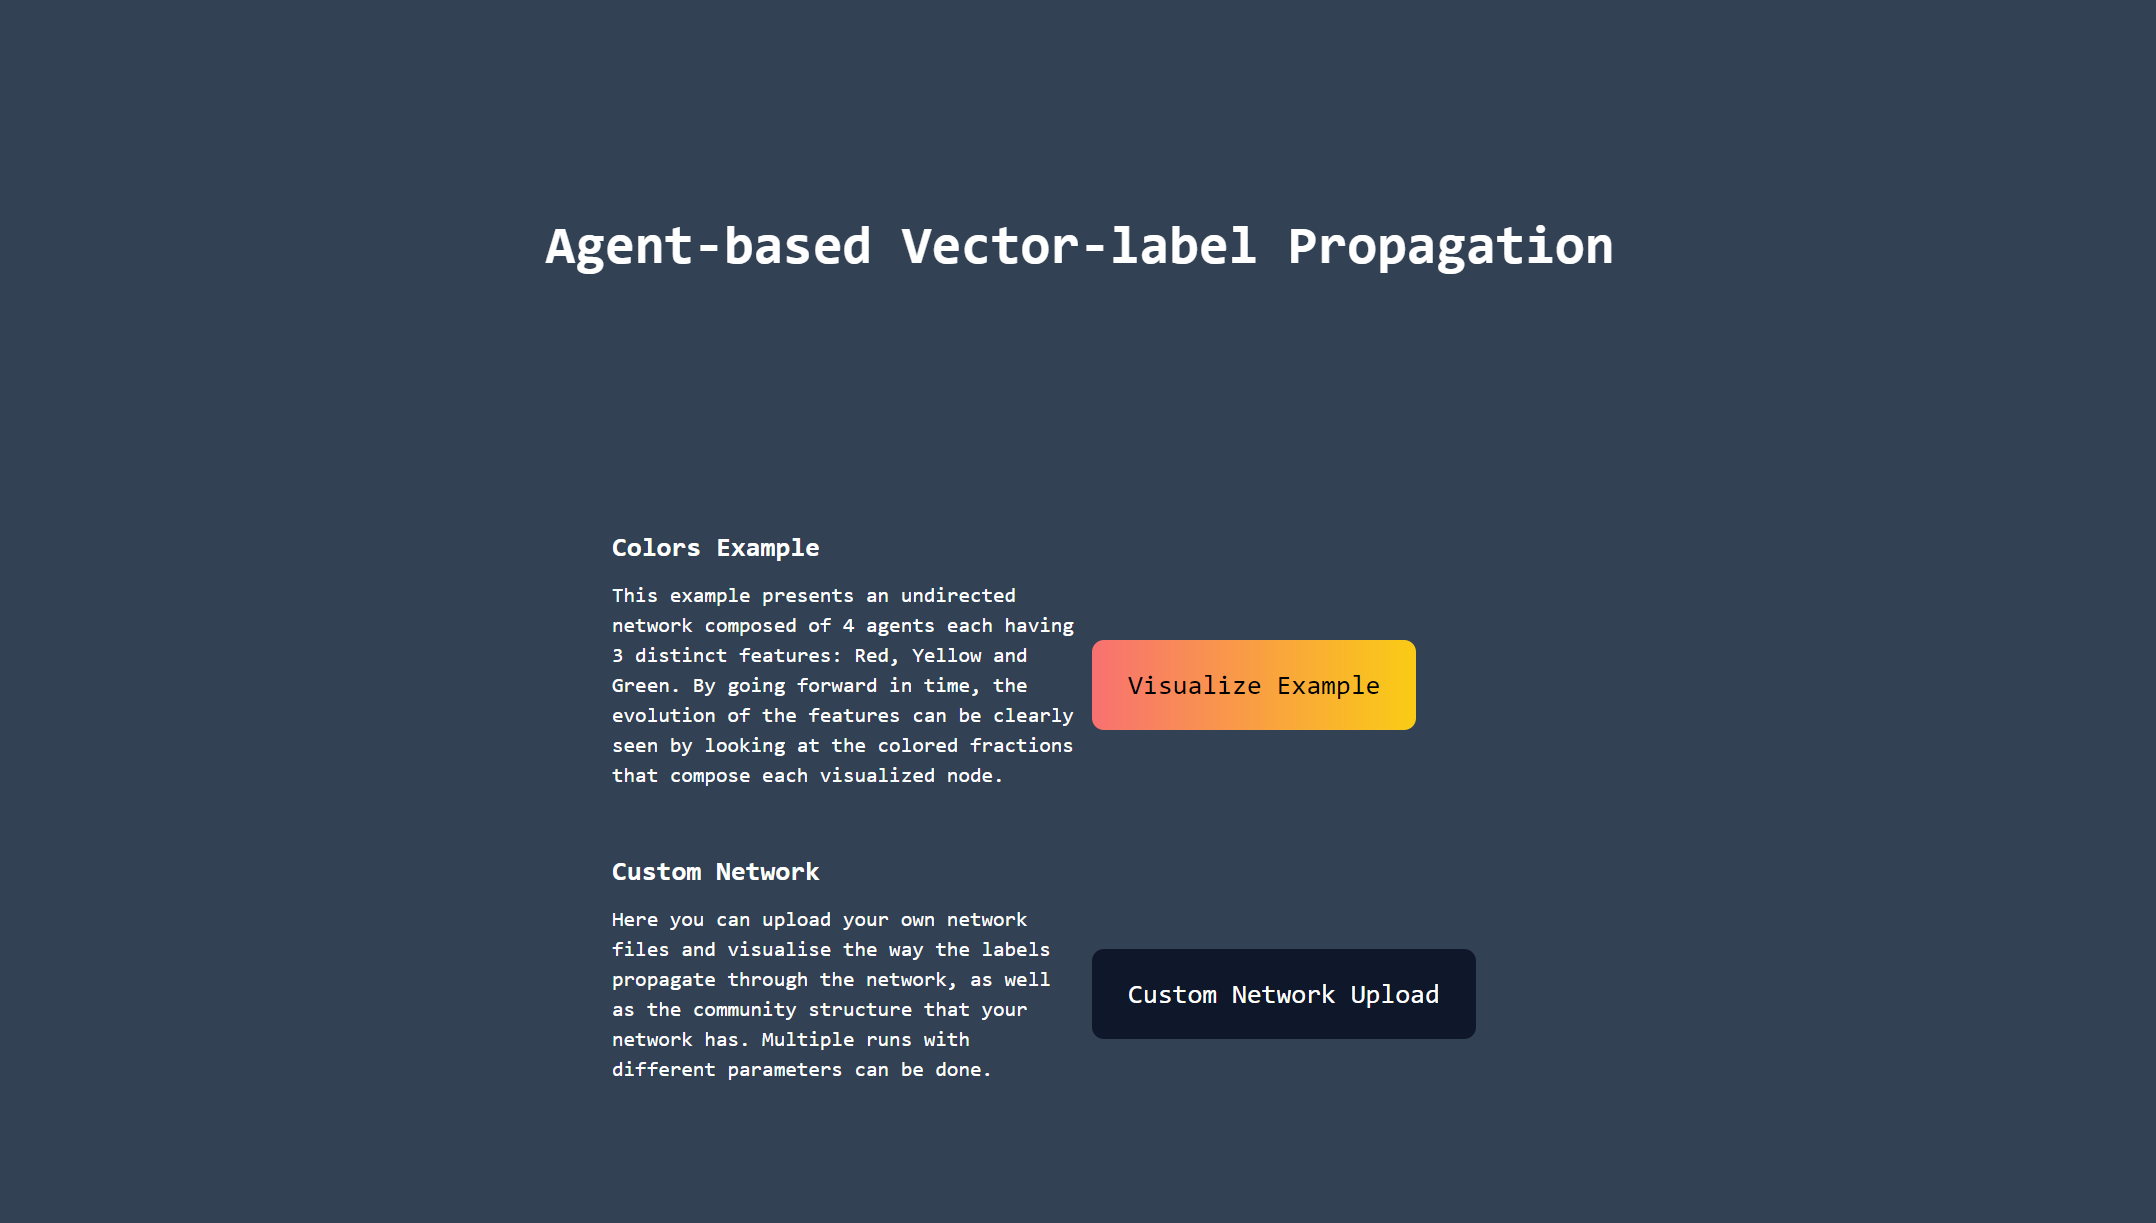
\includegraphics[width=0.9\linewidth,keepaspectratio]{paginaprincipale}
			\caption{Pagina Principale}
			\end{figure}
			\end{center}

			\subsubsection{Esempio Colori}

			La pagina dell'esempio colori, che si puo raggiungere premendo il bottone "Visualize Example" vicino a "Colors Example" sulla pagina principale, ha tutte le funzionalita dell'applicazione, dimostrate su un semplice esempio di grafo non diretto con 4 nodi e 3 archi. In questo esempio si puo vedere il modo in cui le ettichete si propagano ad ogni iterazione attraverso i colori. 


			\begin{center}
			\begin{figure}[H]
			\centering
			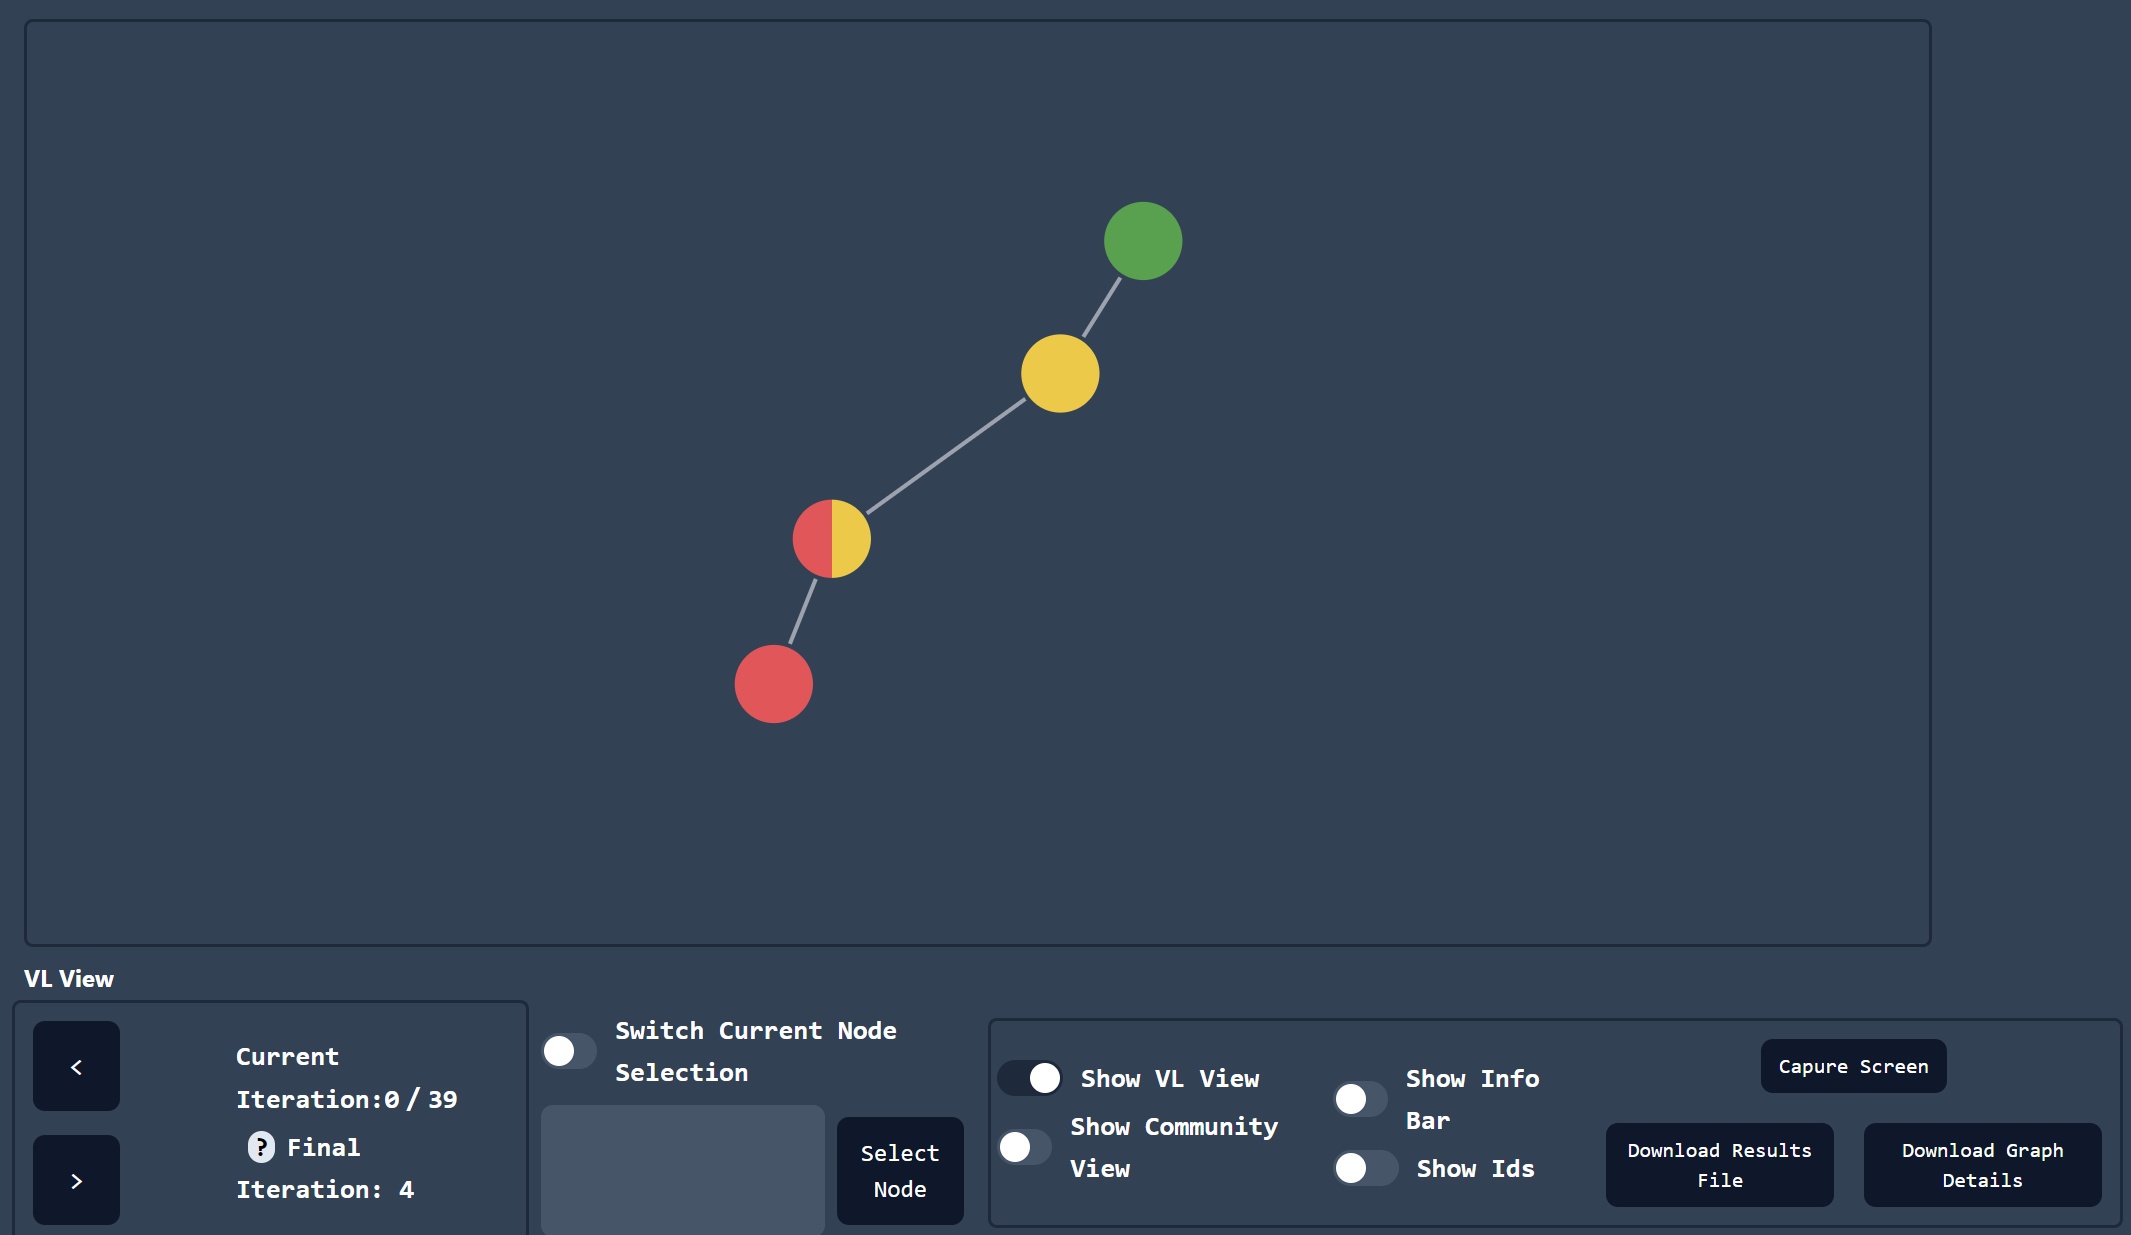
\includegraphics[width=0.9\linewidth,keepaspectratio]{colorsexample}	
			\caption{Esempio Colori}
			\end{figure}
			\end{center}
			I componenti che compongono l'interfaccia di visualizzazione della rete sono:
			\begin{itemize}
			\item \textbf{La bara di controllo} 

			Questo componenente contiene tutte le modalita che si possono usare per controllare la visualizzazione della rete. 

			Iniziando da sinistra e andando verso destra, la bara di controllo contiene per prima cosa un rettangolo con dei tasti per controllare l'iterazione corrente che viene visualizzata, assieme alla iterazione che viene considerata finale dall'algoritmo (nel caso dell'esempio colori, il parametro p viene fissato a 0.1). \par
			\begin{center}
			\begin{figure}[H]
			\centering
			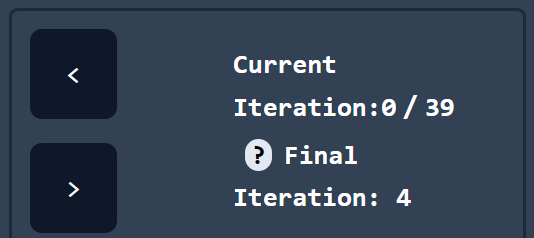
\includegraphics[width=0.9\linewidth,keepaspectratio]{iterationcontrol}
			\caption{Controlli Iterazione}
			\end{figure}
			\end{center}
			La seconda parte della bara di controllo viene utilizzata per cambiare il modo di selezione nodo e per cercare un nodo specifico nella rete. Se si preme il tasto per cambiare il modo di selezione nodo, si puo selezionare un secondo nodo, in modo che, ulteriormente, si possono comparare i vettori di ettichete dei due nodi specifici. La bara di ricerca di un nodo specifico diventa molto utile nel caso in cui la rete utilizzata ha molti nodi e quindi dove la selezione del nodo dalla rete diventa difficile. \par
			\begin{center}
			\begin{figure}[H]
			\centering
			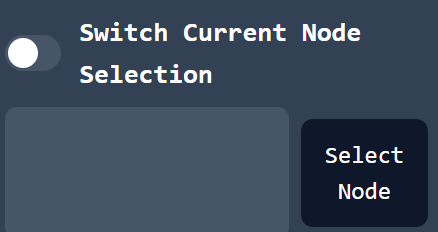
\includegraphics[width=0.9\linewidth,keepaspectratio]{nodeselection}
			\caption{Controlli Selezione Nodo}
			\end{figure}
			\end{center}
			L'ultima parte della bara di controllo contiene alcuni controlli per cambiare il layout di visualizzazione e alcuni tasti per: catturare la configurazione corrente dell'applicazione, scaricare il file dei risultati, scaricare il file contenente i dettagli del grafo e scaricare un file contenente la comparazione tra due nodi selezionati. Le opzioni per cambiare la configurazione dell'applicazione sono: Show VL View (che viene utilizzato per nascondere o per visualizzare la View che presenta graficamente la configurazione dei vettori d'ettichete), Show Community View (che viene utilizzato per nascondere o per visualizzare la View che presenta graficamente la divisione in communita della rete), Show Info Bar (che viene utilizzato per nascondere e far comparire la bara laterale che presenta le informazioni sulla rete, o sui nodi selezionati) e Show Ids (che viene utilizzato per nascondere o per visualizzare gli ID all'interno di ogni nodo in una View). 

			Formato Graph Details 

			Formato Comparazione nodi 

			\begin{center}
			\begin{figure}[H]
			\centering
			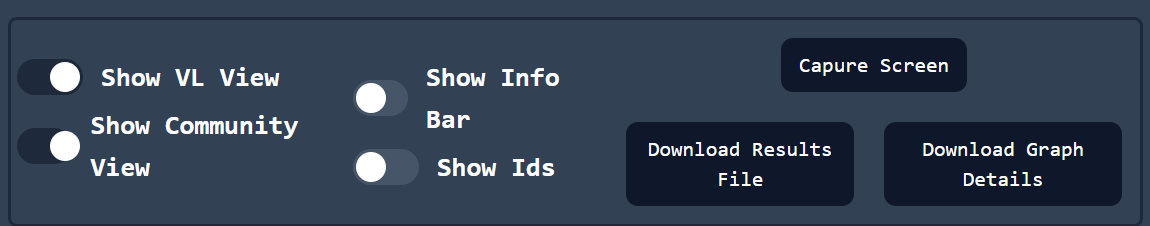
\includegraphics[width=0.9\linewidth,keepaspectratio]{viewcontrol}
			\caption{Controlli Vista}
			\end{figure}
			\end{center}
			\item \textbf{VL View} 

			La VL View rappresenta la vista che visualizza la rete dal punto di vista dei vettori delle ettichete. Tutti i belonging coefficient sommano a 1 e quindi ogni etticheta viene rappresentata da un colore che occupa la percentuale specifica sul nodo (per esempio se un'etticheta su un nodo ha il belonging coefficient uguale a 0.5, allora il colore di quell'etticheta occupera 50\% del nodo nella VL View). 
			
			\begin{center}
			\begin{figure}[H]
			\centering
			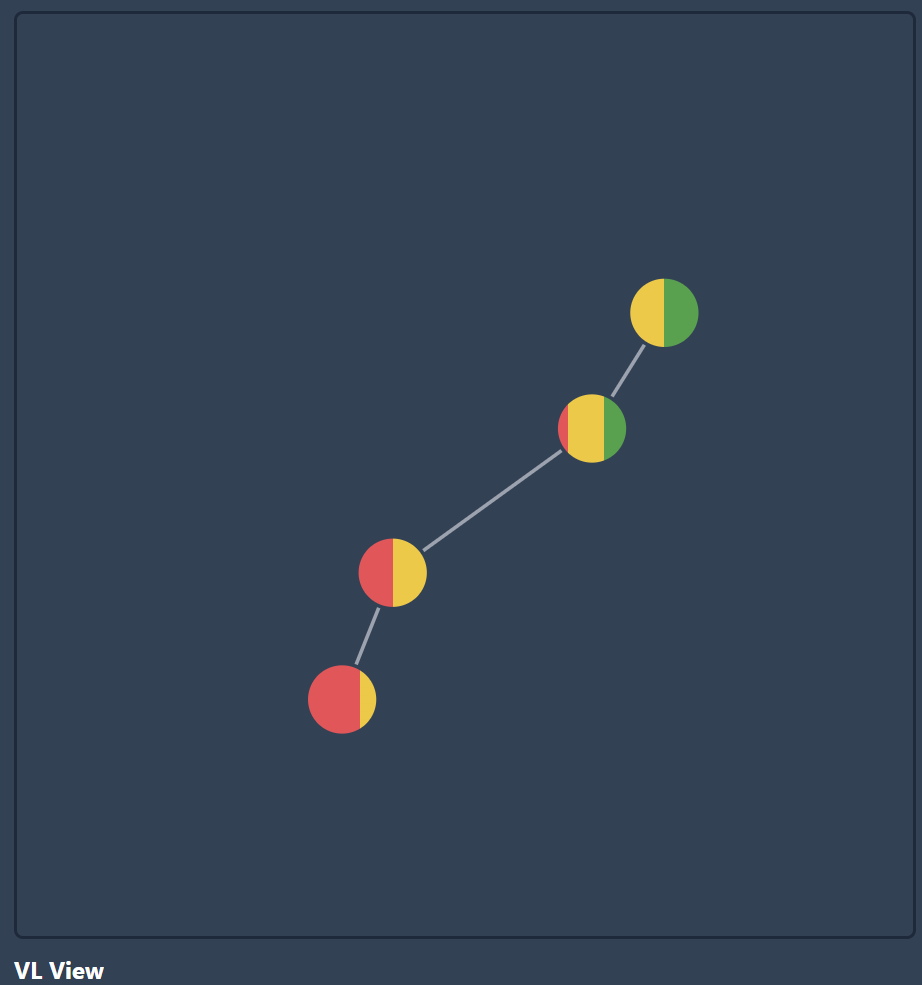
\includegraphics[width=0.9\linewidth,keepaspectratio]{vlview}
			\caption{Vista Vettori di ettichete}
			\end{figure}
			\end{center}

			\item \textbf{Community View} 

			La Community View rappresenta la vista che visualizza la rete dal punto di vista delle communita che compongono la rete. I nodi che si trovano nella stessa communita avrano lo stesso colore, in modo da identificare facilmente i nodi appartenenti alla stessa communita dal punto di vista strutturale. La communita di ogni nodo puo essere conosciuta dalle informazioni specifiche di ogni nodo, quando esso viene selezionato. 

			\begin{center}
			\begin{figure}[H]
			\centering
			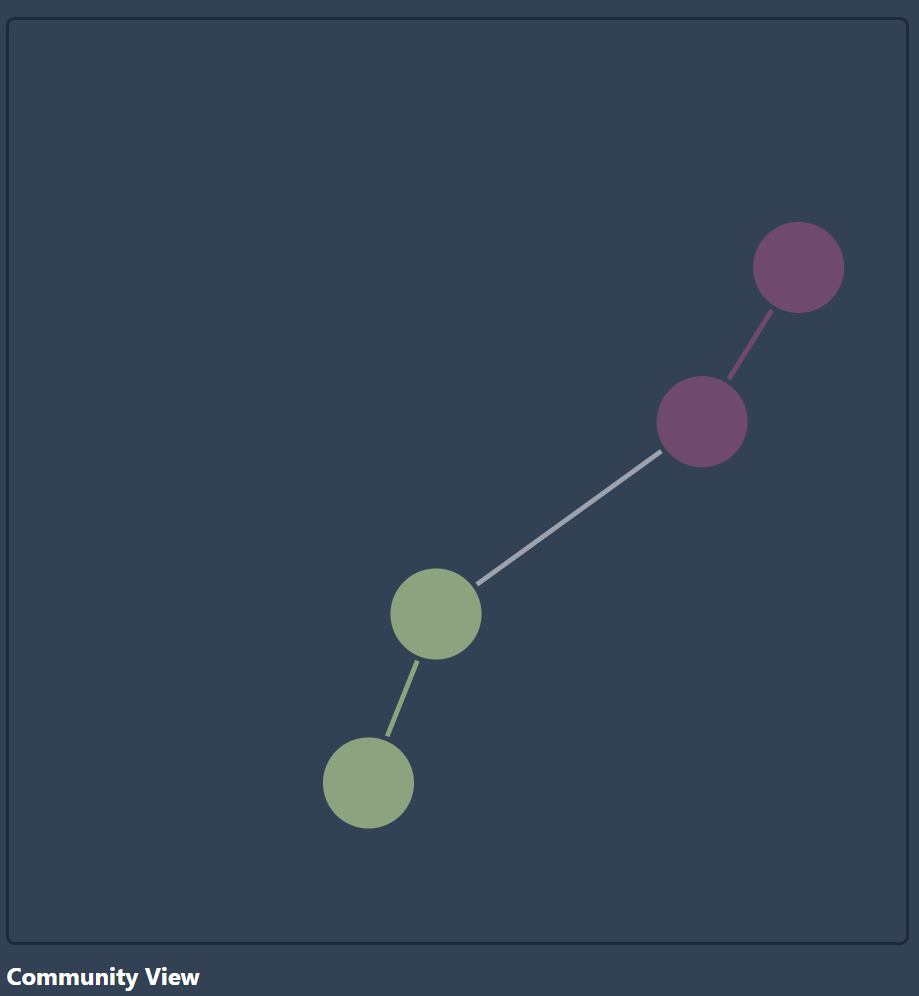
\includegraphics[width=0.9\linewidth,keepaspectratio]{comview}
			\caption{Vista Communita}
			\end{figure}
			\end{center}

			\item \textbf{Info Bar} 

			La Info Bar visualizza, nel caso nessun nodo viene selezionato, le informazioni generali riguardanti la rete, come tipo di rete, numero di nodi, numero di archi e diametro. Nel caso in cui un nodo viene selezionato, la bara delle informazioni mostra il grado di quel nodo, la communita appartenente, assieme al suo colore e il vettore delle ettichete coi belonging coefficient di ogni etticheta, assieme al colore dell'etticheta. Nel caso in cui due nodi vengono selezionati, ci saranno due bare di informazioni che mostrano le stesse informazioni di prima per entrambi i nodi. 

			\begin{center}
				\begin{figure}[H]
				\centering
				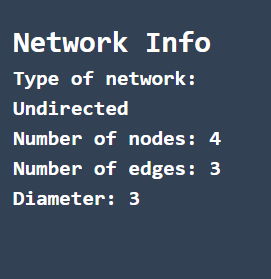
\includegraphics[width=0.4\linewidth]{infobargeneral}
				\caption{Barra Informazioni senza un nodo selezionato}
				\end{figure}
				\begin{figure}[H]
				\centering
				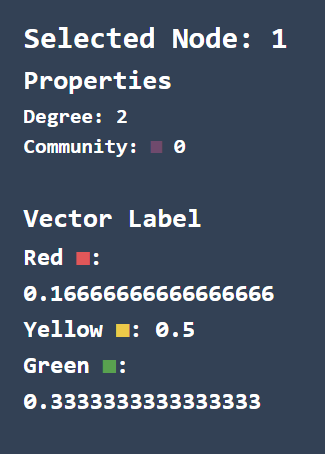
\includegraphics[width=0.4\linewidth]{infobar1}
				\caption{Barra Informazioni con un solo nodo selezionato}
				\end{figure}
				\begin{figure}[H]
				\centering
				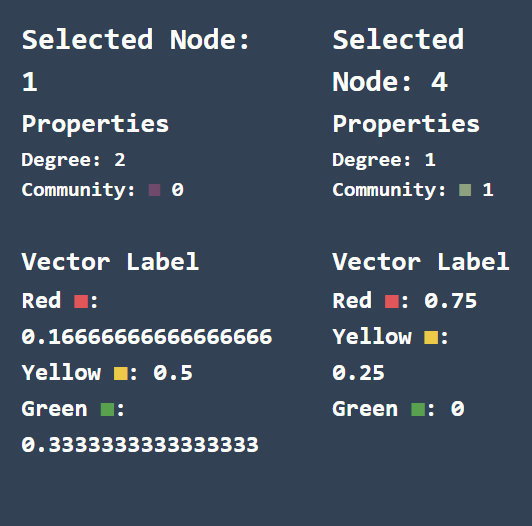
\includegraphics[width=0.6\linewidth]{infobar2}
				\caption{Barra Informazioni con due nodi selezionati}
				\end{figure}
			\end{center}
			\end{itemize}
			
			\subsubsection{Pagina Caricamento Reti Sociali Personalizzate}
			Nel caso della pagina di upload delle reti sociali personalizzate, l'utente puo caricare i suoi dataset personali, formattati in un formato descritto nella pagina stessa, e visualizzare i risultati di AVPRA sulla sua rete. 

			L'utente ha la possibilita di personalizzare diverse opzioni riguardanti l'interpretazione dei dati e i parametri con cui l'algoritmo sara eseguito. 

			I file riguardanti la rete che l'utente puo caricare sull'applicazione sono i seguenti:

			\begin{itemize}
				\item Il file degli archi che dev'essere un file .csv col seguente formato: 

				\begin{equation}
				\dots \\
				nodo1\ nodo2\ \{ peso \} \\
				\dots
				\end{equation}

				Questo formato mostra che il nodo1 e collegato al nodo2 e che l'arco ha il peso specificato. Il peso e opzionale e quindi il file puo essere definito anche nel seguente modo: 

				\begin{equation}
				\begin{aligned}
				\dots \\
				nodo1\  nodo2 \\
				nodo2\  nodo4 \\
				\dots
				\end{aligned}
				\end{equation}				

				\item Il file dei vettori delle ettichete con cui i nodi vengono inizializzati. 

				Questo file dev'essere un file .csv col seguente formato: 

				\begin{equation}
				\begin{aligned}
				b_1(l_1);\ b_1(l_2);\ \dots;\ b_1(l_k) \\
				b_2(l_1);\ b_2(l_2);\ \dots;\ b_2(l_k) \\
				b_3(l_1);\ b_3(l_2); \dots;\ b_3(l_k) \\
				\dots
				\end{aligned}
				\end{equation}
				
				In questo caso $b_1, b_2, b_3, \dots$ sono le funzioni del belonging coefficient dei nodi $1, 2, 3, \dots$ e $l_1, l_2, \dots, l_k$ sono le ettichete della rete. Tutti i valori di ogni riga devono sommare a 1. 
				

				\item Il file dei nomi delle ettichete che dev'essere un file .csv col seguente formato: 

				\begin{equation}
				l_1;\ l_2;\ l_3;\ l_4;\ \dots
				\end{equation}

				\item Il file dei colori con cui vengono rappresentate le ettichete. 

				Questo file dev'essere un file .csv che ha il seguente formato: 

				\begin{equation}
				hex_1;\ hex_2; \dots
				\end{equation}
				In questo formato $hex_1, hex2, \dots$ sono i codici essadecimali dei colori con cui saranno rappresentate le ettichete $l_1, l_2, \dots$ nella visualizzazione. 

				Un'esempio del formato di questo file e: 

				\begin{equation}
				\#433A3F;\ \#404A56;\ \#3D5A6C;\ \#58827E;\ \#659687; \dots
				\end{equation}
			\end{itemize}
			Le opzioni che l'utente puo scegliere sono le seguenti:
			\begin{itemize}
				\item Grafo diretto o non diretto 

				Quest'opzione permette all'utente di scegliere se il grafo costruito dal file degli archi viene interpretato come un grafo diretto o non diretto.

				\item Propagazione ettichete dai predecessori o successori 

				Quest'opzione permette all'utente di scegliere se la propagazione delle ettichete viene influenzata dagli nodi entranti o dagli nodi uscenti. Nel caso in cui il grafo viene interpretato come un grafo non diretto, quest'opzione non e disponibile.

				\item Negligibly Threshold 

				Quest'opzione permette all'utente di scegliere il valore del parametro negligibly threshold associato all'algoritmo, da cui dipende l'iterazione finale dell'algoritmo.

				\item Numero di iterazioni 

				Quest'opzione permette all'utente di scegliere il numero di iterazioni per cui l'algoritmo sara eseguito.

				\item Formula per il peso nella funzione di aggiornamento 

				Quest'opzione permette all'utente di scegliere una formula (dipendente dal numero di vicini del nodo) per i pesi nella funzione di aggiornamento dell'algoritmo AVPRA.

			\end{itemize}
			
			\subsubsection{Esempio Personalizzato}

			Nel caso dell'esempio personalizzato, l'interfaccia utente e pratticamente uguale all'interfaccia presente nell'Esempio Colori, con qualche piccola differenza data dalle opzioni che l'utente ha scelto nella fase di caricamento della rete.

			\paragraph*{La bara di informazioni} si comporta nello stesso modo della bara di informazioni dell'Esempio Colori, ma offre piu informazioni generali riguardo la rete caricata sull'applicazione.
			
			\begin{center}
				\begin{figure}[H]
				\centering
				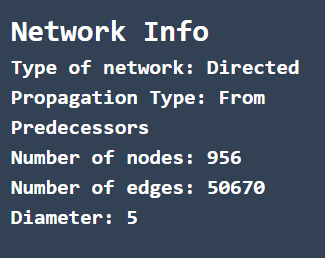
\includegraphics[width=0.5\linewidth]{infobargeneralcustom}
				\caption{Barra Informazioni Generale per una rete diretta e con propagazione delle ettichete da predecessori}
				\end{figure}
				\begin{figure}[H]
				\centering
				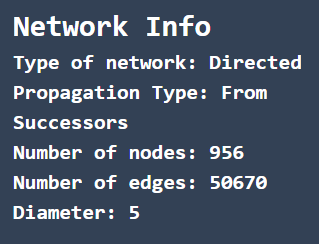
\includegraphics[width=0.5\linewidth]{infobargeneralcustomdirectedsuccessors}
				\caption{Barra Informazioni Generale per una rete diretta e con propagazione delle ettichete da successori}
				\end{figure}
				\begin{figure}[H]
				\centering
				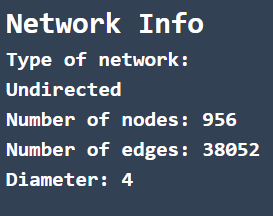
\includegraphics[width=0.5\linewidth]{infobargeneralcustomundirected}
				\caption{Barra Informazioni Generale per una rete non diretta}
				\caption{Barra Informazioni Senza Nodo Selezionato}
%				\includegraphics[width=0.5\linewidth]{infobar1custom}
%				\caption{Barra Informazioni con un solo nodo selezionato}
%				\includegraphics[width=0.3\linewidth]{infobar2custom}
%				\caption{Barra Informazioni con due nodi selezionati}
				\end{figure}
			\end{center}

			\paragraph*{La bara di controllo} subisce modifiche solo nella sezione di Controlli Iterazione. In questo caso, il numero massimo delle iterazioni viene sostituito col numero di iterazioni scelto dall'utente durante il caricamento della rete, e l'iterazione finale cambia in modo che il numero d'ordine mostrato sia l'iterazione dove avviene la condizione di terminazione.

			\begin{center}
				\begin{figure}[H]
				\centering
				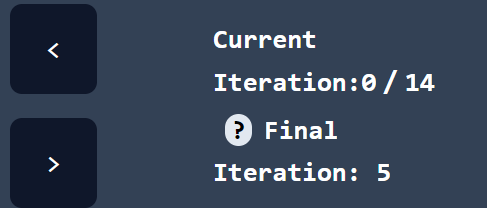
\includegraphics[width=0.5\linewidth]{iterationcontrolcustom}
				\caption{Controlli Iterazione per reti personalizzate}
				\end{figure}
			\end{center}
\chapter{Sviluppi Futuri}
	Discussione riguardo il deployment dell'applicazione.
\chapter{Conclusioni}

%
%			BIBLIOGRAFIA
%
\begin{thebibliography}{0}
%
\bibitem{mapequationsite}
https://www.mapequation.org/infomap/

\bibitem{mapequationnavigatorsite}
https://www.mapequation.org/navigator/

\bibitem{snaintro}
https://towardsdatascience.com/social-network-analysis-from-theory-to-applications-with-python-d12e9a34c2c7

\bibitem{avpra}
Valerio Bellandi, Paolo Ceravolo, Ernesto Damiani, and Samira Maghool: Agent-based Vector-label Propagation for Explaining Social Network Structures. In: Springer Verlag (Lecture Notes in Communications in Computer and Information Science (CCIS)) (2022)

\bibitem{raghavan}
Raghavan, U.N., Albert, R., Kumara, S.: Near linear time algorithm to detect
community structures in large-scale networks. Physical review E 76(3), 036106
(2007)

\bibitem{componentireact}
https://it.reactjs.org/docs/react-component.html

\bibitem{tipicomponenti}
https://it.reactjs.org/docs/components-and-props.html

\bibitem{statoreact}
https://it.reactjs.org/docs/state-and-lifecycle.html

\bibitem{jsxreact}
https://it.reactjs.org/docs/introducing-jsx.html

\bibitem{hooksreact}
https://it.reactjs.org/docs/hooks-intro.html

\bibitem{typescript}
https://www.typescriptlang.org/

\bibitem{typescripthandbook}
https://www.typescriptlang.org/docs/handbook/typescript-in-5-minutes-func.html

\bibitem{nextjs}
https://nextjs.org/learn/foundations/about-nextjs/what-is-nextjs

\bibitem{d3js}
https://d3js.org/

\bibitem{katex}
https://www.npmjs.com/package/katex

\bibitem{tailwindcss}
https://tailwindcss.com/

\bibitem{flaskforeword}
https://flask.palletsprojects.com/en/2.1.x/foreword/

\bibitem{flask}
https://flask.palletsprojects.com/en/2.1.x/

\bibitem{sympy}
https://www.sympy.org/en/index.html

\bibitem{cdlib}
https://cdlib.readthedocs.io/en/latest/
%
\end{thebibliography}
% 
\end{document}


 
